\subsection{Geometric examples of homology classes}
% \begin{flushright}
%  \textit{An meinen Doktorvater Herr B\"{o}digheimer}
% \end{flushright}

In this subsection we consider the case $g=2$, hence $\S$ denotes the surface $\Sigma_{2,1}$.
We construct some homology classes in $H_2(C_2(\S))$: our aim is to get a first understanding
of why this homology group is isomorphic to $\Sym_2(\H)=\H^{\otimes 2}/\mathfrak{S}_2$.

In the following $c$ and $d$ will always denote two simple closed curves on $\S$, with corresponding homology classes $[c],[d]\in\H$.
\begin{ex}
 \label{ex:one}
Suppose that $c$ and $d$ are as in Figure \ref{fig:exampleone}: $c$ and $d$ are disjoint and non-separating.
We can consider inside $C_2(\S)$
the torus $c\times d$ of configurations in which one of the two points runs along $c$, while the other runs
along $d$. We associate to the fundamental class $\tau_1\in H_2(C_2(\S))$ of this torus the tensor product $[c]\otimes[d]\in\H^{\otimes 2}$.

Since our configurations are unordered and since we work with coefficients in $\Z_2$, the same
class $\tau_1$ can be obtained as a tensor product $[d]\otimes[c]$, i.e. exchanging the order of the two
curves: we can neglect the sign $-1$ that this operation would generate. We represent $\tau_1$ as $[c]\cdot[d]\in\Sym_2(\H)$.
\end{ex}
\begin{figure}[h]\centering
 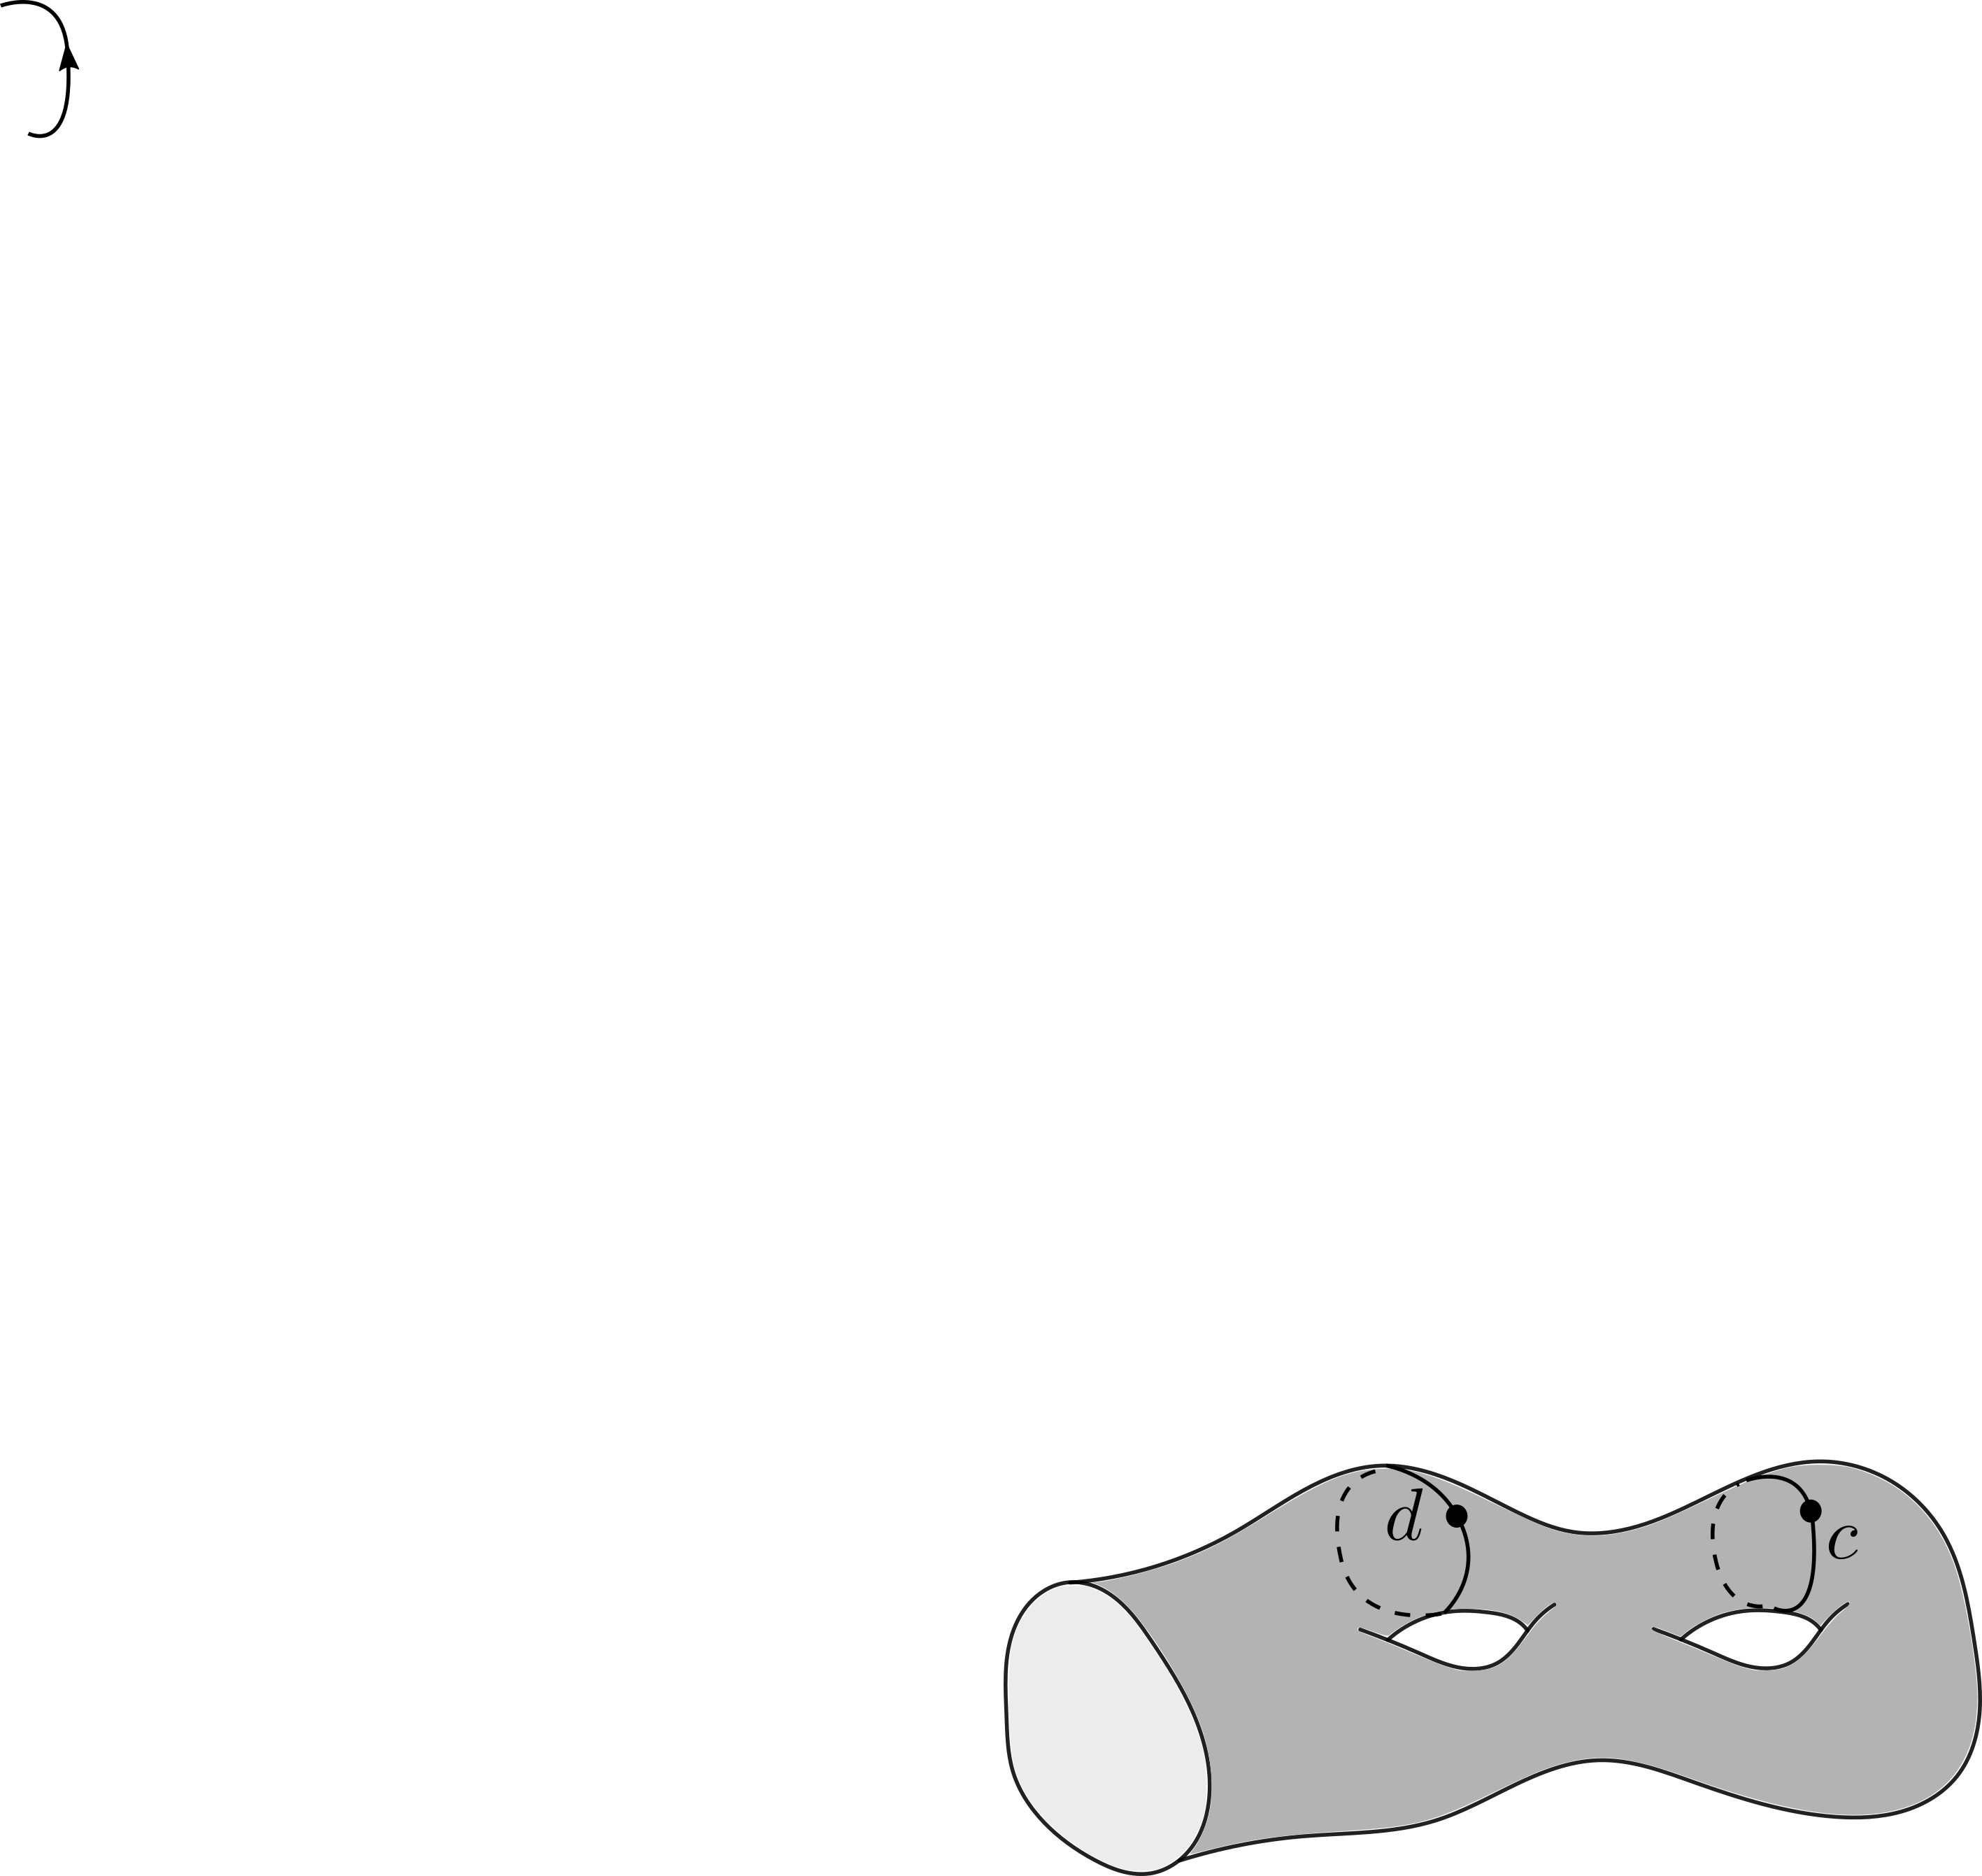
\includegraphics[scale=1.0]{figures/exampleone.pdf}
 \caption{}
\label{fig:exampleone}
\end{figure}

\begin{ex}
 \label{ex:two}
Suppose that $c$ and $d$ are as in Figure \ref{fig:exampletwo}:
$c$ and $d$ are disjoint, and
 $c$ bounds a subsurface $\check{\S}$ of $\S$ (the shaded region), such that $d$ is not contained in $\check{\S}$.
 
 Then the homology class $\tau_2=[c]\cdot[d]$ vanishes, because the torus $c\times d$ is the boundary in $C_2(\S)$
 of the 3-manifold $\check{\S}\times d$ containing all configurations in which one point lies on $\check{\S}$ and
 the other on $d$. This is consistent with the representation $\tau_2=[c]\cdot[d]$, because $[c]=0\in \H$.
\end{ex}
\begin{figure}[h]\centering
 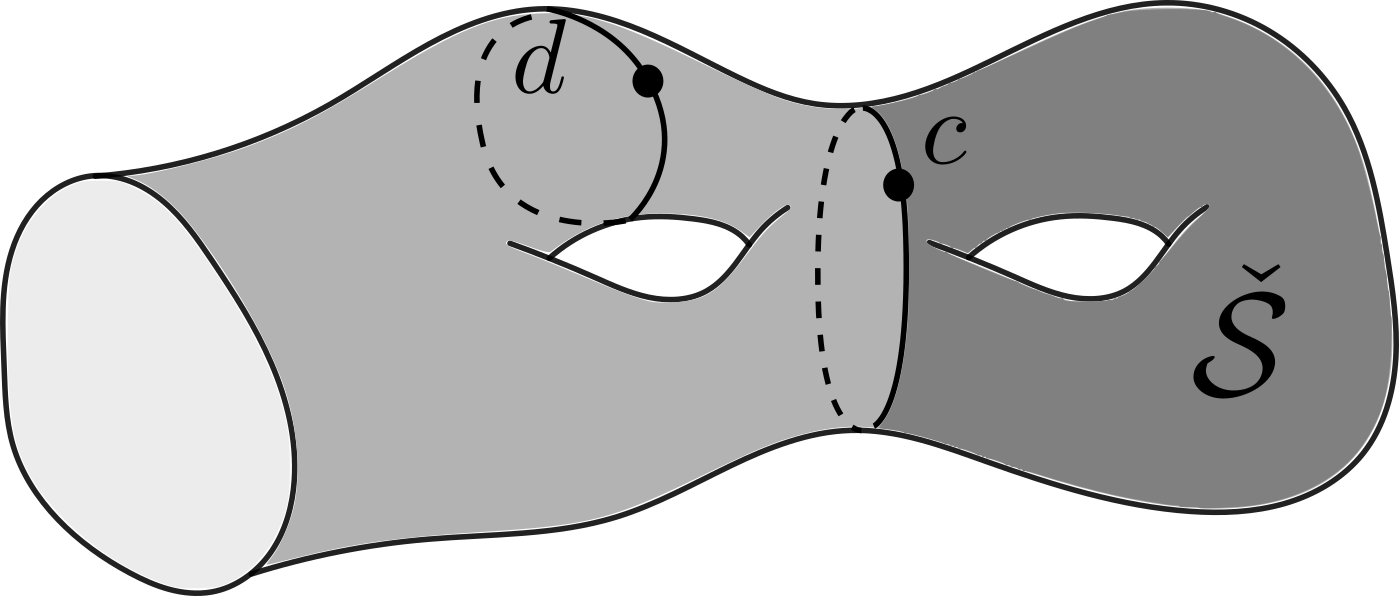
\includegraphics[scale=1.0]{figures/exampletwo.pdf}
 \caption{}
\label{fig:exampletwo}
\end{figure}

\begin{ex}
 \label{ex:three}
 Suppose that $c$ and $d$ are as in Figure \ref{fig:examplethree}: $c$ and $d$ are non-separating and 
intersect transversely in one point $P\in\S$. In this case the torus $c\times d$ is a subspace
of $\SP^2(\S)$, but $c\times d$ is not contained in $C_2(\S)$ as in Example \ref{ex:one}.

To solve this problem, we consider a small open neighborhood $P\in \U\subset\S$, and we remove from the torus $c\times d$
all configurations in which both points lie in $\U$: these removed configurations form an open disc inside the torus $c\times d$.

We obtain an embedding $\Sigma_{1,1}\hookrightarrow C_2(\S)$;
the boundary $\partial\Sigma_{1,1}$,
seen as a curve in $C_2(\S)$, is homotopic to a curve $\gamma$ in which one point spins $360^{\circ}$ around the other.
We note that the curve $\gamma\subset C_2(\S)$ is homotopic to a double covering of a curve $\gamma'\subset C_2(\S)$,
in which the two points exchange their positions after spinning $180^{\circ}$ around each other. All curves
$\partial\Sigma_{1,1}$, $\gamma$, $\gamma'$ and the homotopies relating them
are supported on the closure of $C_2(\U)$ in $C_2(\S)$.

We can therefore find a map from a M\"{o}bius band $\M$ to the closure of $C_2(\U)$ in $C_2(\S)$,
such that the images of the curves $\partial\M$ and $\partial\Sigma_{1,1}$ in $C_2(\S)$ coincide.
The union $\Sigma_{1,1}\cup_{\partial}\M$ along the boundary is then a closed
non-orientable surface of genus $3$, i.e. the connected sum of a torus and a projective plane.

The surface $\Sigma_{1,1}\cup_{\partial}\M$ is equipped with a map to $C_2(\S)$, hence its fundamental class with coefficients
in $\Z_2$ yields a homology class $\tau_3\in H_2(C_2(\S))$; thus we have managed to adapt
the construction from Example \ref{ex:one} to the case of two intersecting curves. We represent $\tau_3$
as $[c]\cdot[d]\in\Sym_2(\H)$.
\end{ex}
\begin{figure}[h]\centering
 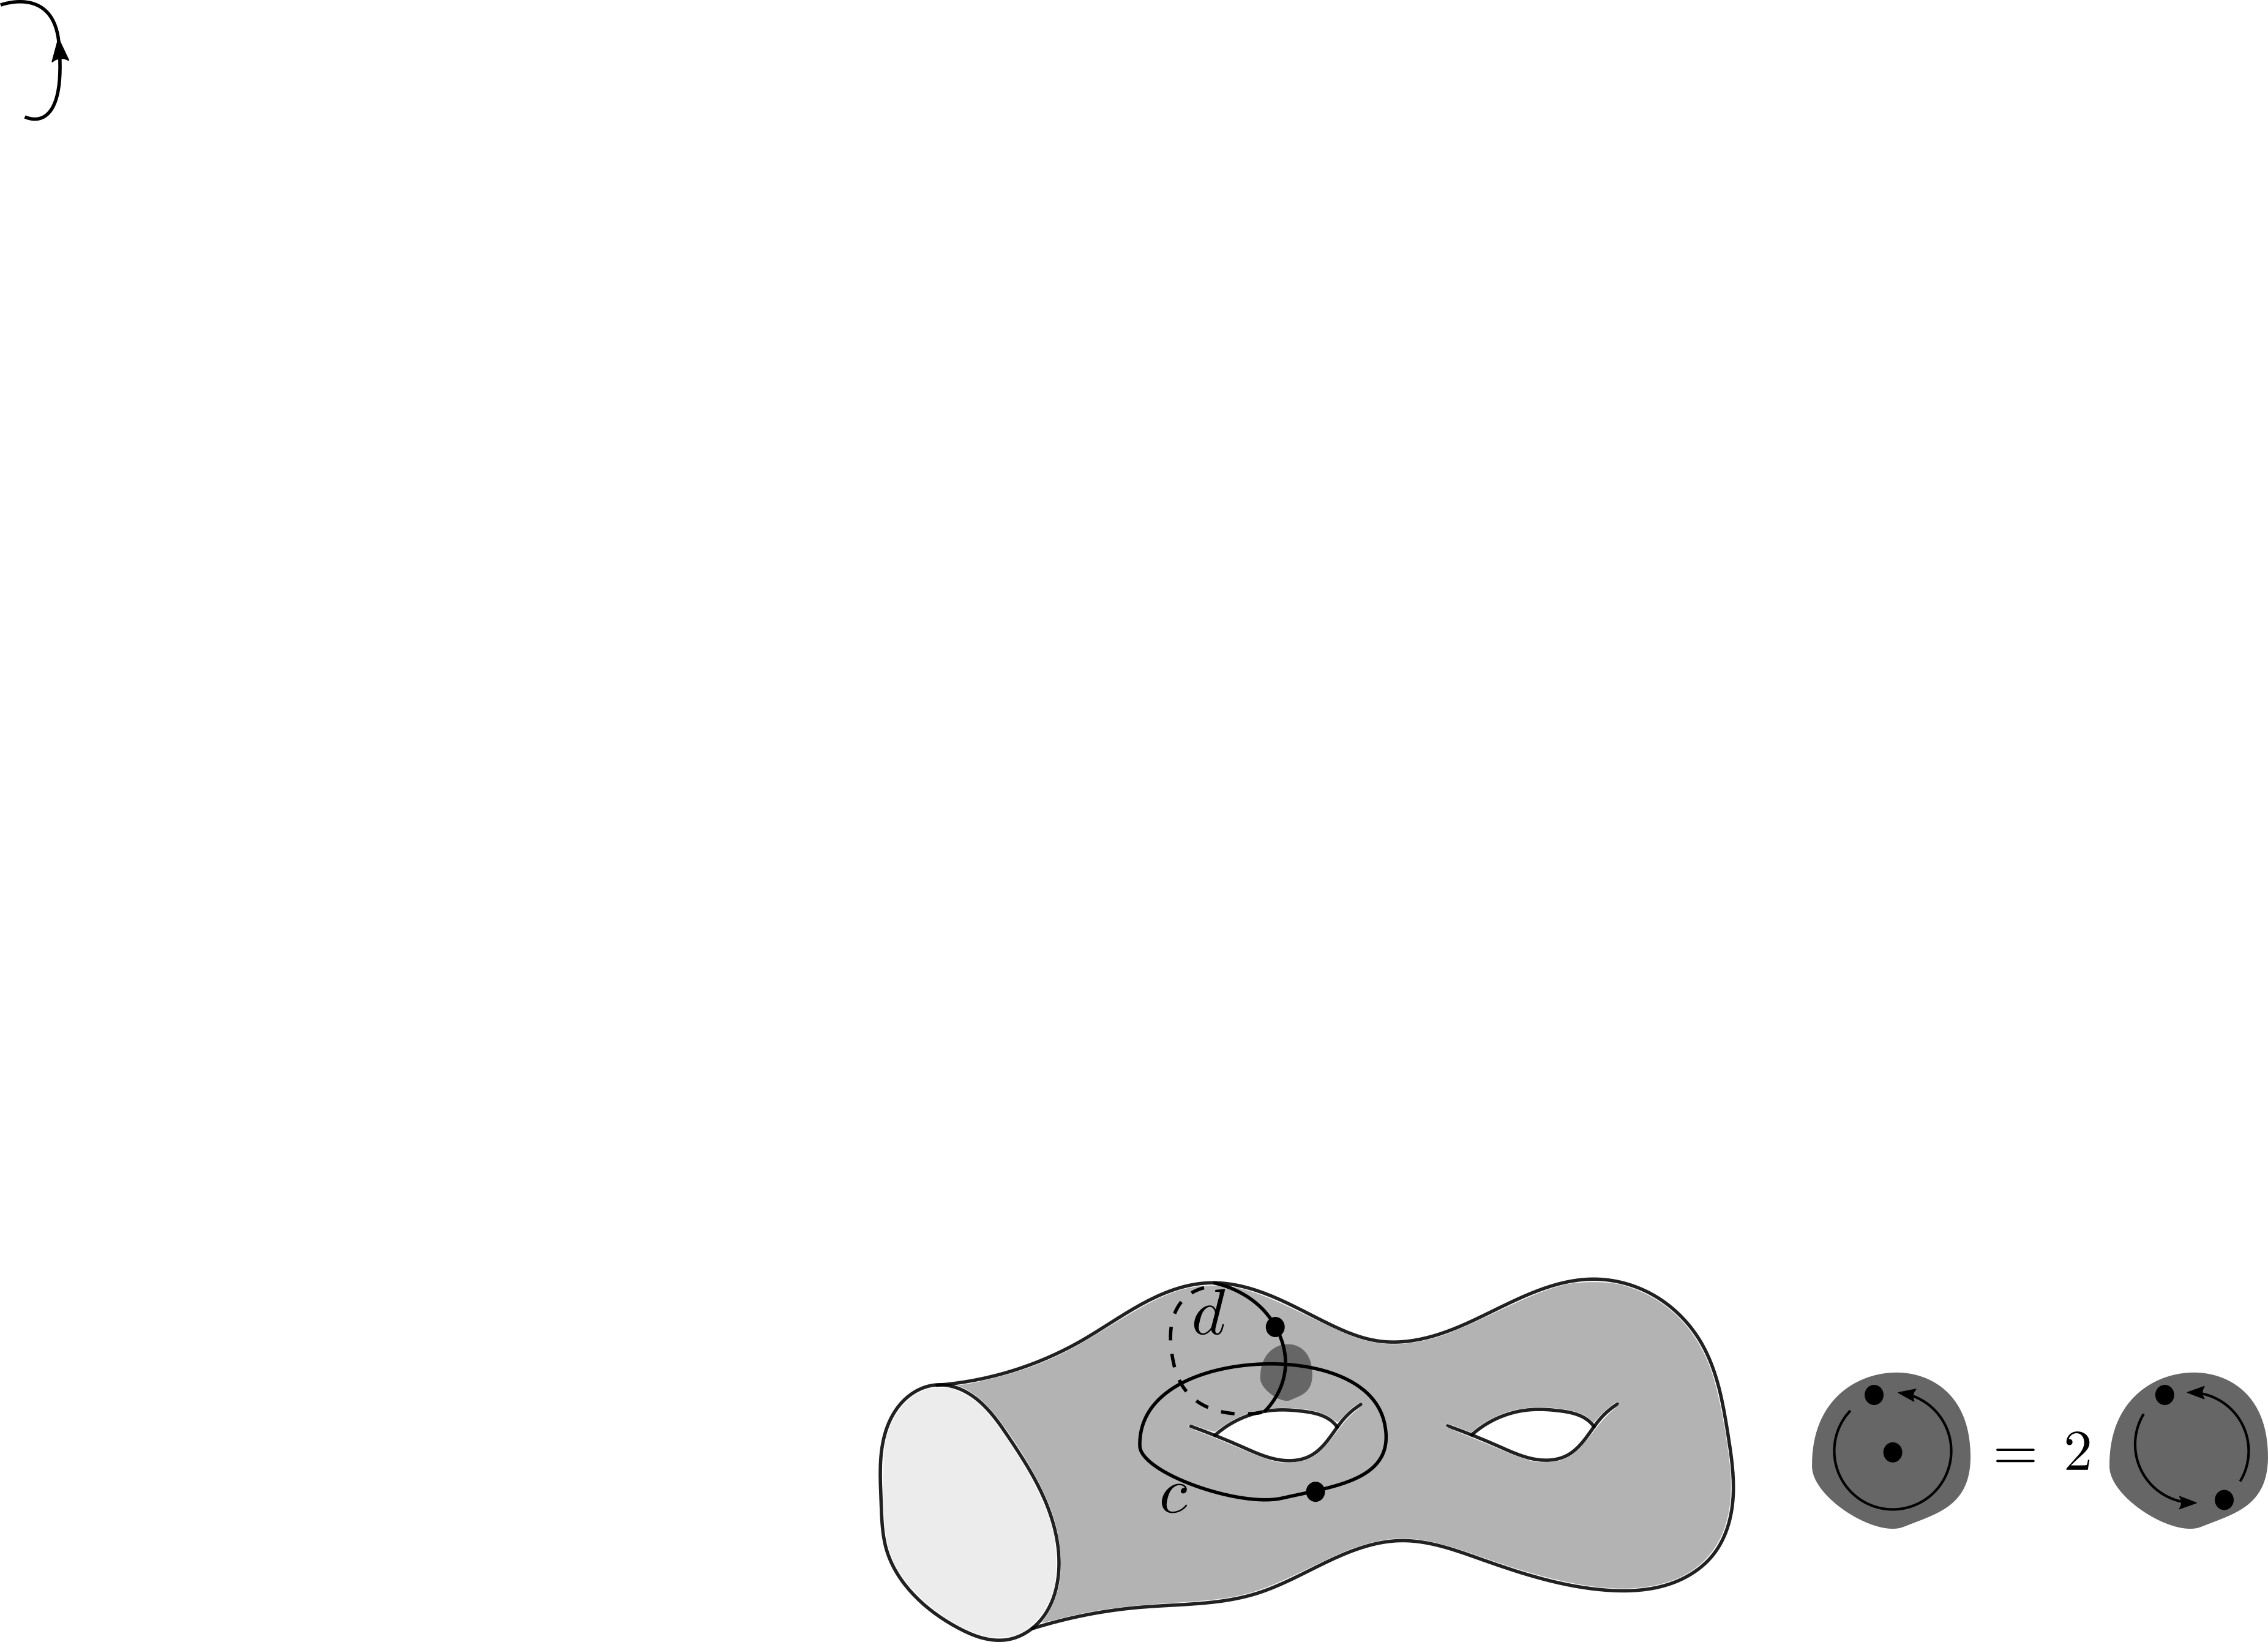
\includegraphics[scale=1.0]{figures/examplethree.pdf}
 \caption{}
\label{fig:examplethree}
\end{figure}

\begin{ex}
 \label{ex:four}
 Suppose that $c$ and $d$ are as in Figure \ref{fig:examplefour}: $c$ and $d$ are disjoint, and
 $c$ bounds a subsurface $\check{\S}$ of $\S$ (the shaded region), such that $d$ is contained in $\check{\S}$.
 
 The torus $c\times d$ is contained in $C_2(\S)$, but it is not obvious, at first glance, why its corresponding homology
 class $\tau_4\in H_2(C_2(\S))$ should vanish: the argument used in Example \ref{ex:two} does not work immediately, because the
 3-manifold $\check{\S}\times d$ is only contained in $\SP^2(\S)$ and not in $C_2(\S)$.
 
 We try to modify this 3-manifold in the same spirit of Example \ref{ex:three}. Let $\U\tilde{\times} d\subset \check{\S}\times d$
 be an open tubular neighborhood of $d\times d$: note that this tubular neighborhood is a trivial bundle over
 $d$ with fiber an open disc $\U$. The notation $\tilde{\times}$ means that abstractly we are dealing with a product $\U\times d$,
 but not geometrically: fibers over different points of $d$ are naturally identified with different discs in $\check{\S}$.
 
 We consider the 3-manifold $\check{\S}\times d\setminus \U\tilde{\times} d$: its boundary is the disjoint union
 of the torus $c\times d$ and the torus $\partial \pa{\U\tilde{\times} d}$. The latter torus contains configurations of
 two points in $\S$, one of which spins around $d$, whereas the other is a \emph{satellite} of the first and spins
 around it $360^{\circ}$.
 
 We regard $\partial \U\tilde{\times} d$ as a trivial bundle $\gamma\tilde{\times} d$ over $d$, with fiber the curve $\gamma$
 considered in Example \ref{ex:three}. After a homotopy the latter torus
 becomes a double covering of a torus $\gamma'\tilde{\times} d$: this is a trivial bundle over $d$ with fiber the curve $\gamma'$;
 we can see $\gamma'\tilde{\times} d\subset C_2(\S)$ as a torus of configurations in which the two points
 exchange their positions spinning $180^{\circ}$ around each other, while their barycenter spins around $d$.
 
 We can fill the second boundary of the $3$-manifold $\check{\S}\times d\setminus \U\tilde{\times} d$
 with the product $\M\times d$: the output is a non-orientable $3$-manifold with boundary $c\times d$, witnessing
 that $\tau_4=0$.
 
 This is consistent with the representation $\tau_4=[c]\cdot[d]$, because $[c]=0\in \H$.
\end{ex}

\begin{figure}[h]\centering
 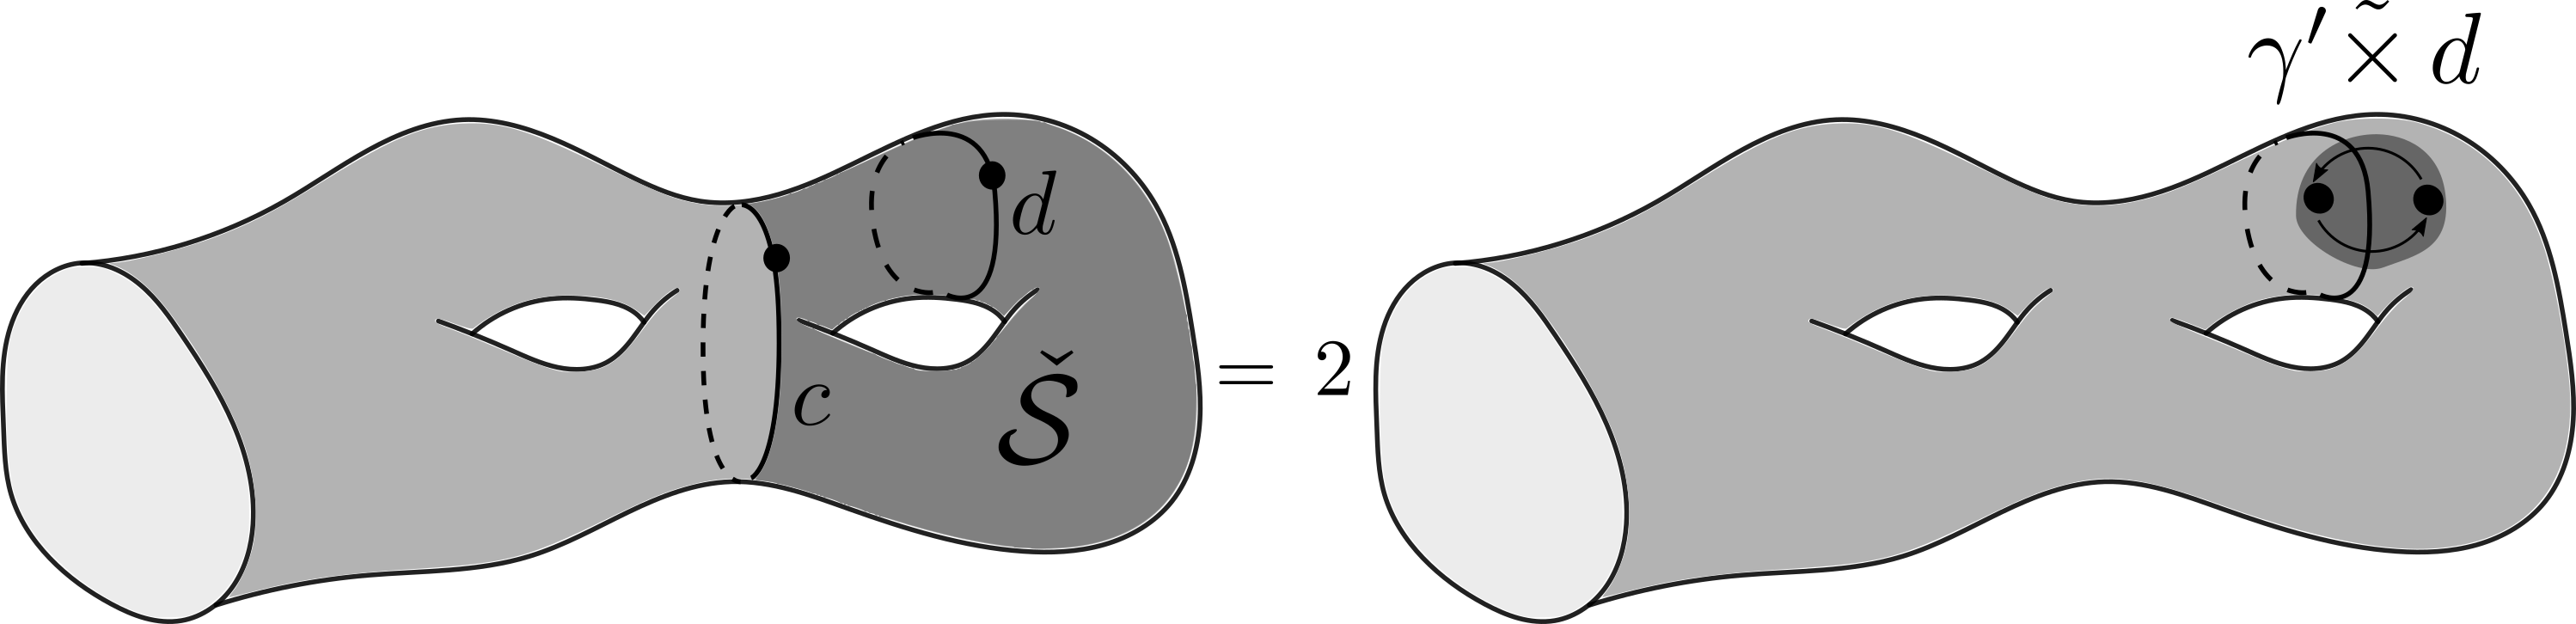
\includegraphics[scale=0.8]{figures/examplefour.pdf}
 \caption{}
\label{fig:examplefour}
\end{figure}

\begin{ex}
 \label{ex:five}
 Suppose that $c$ and $d$ are as in Figure \ref{fig:examplefive}:
 $c$ bounds a subsurface $\check{\S}$, and $d$ is cut by $c$ into two arcs, one of which, denoted by $e$, lies
 in $\check{\S}$.
 
 In this example the complications from Examples \ref{ex:three} and \ref{ex:four} arise at the same time.
 
 To define the class $\tau_5\in H_2(C_2(\S))$, we start with the torus $c\times d$ and we perform two surgeries
 with two different M\"{o}bius bands to solve the two intersections of $c$ and $d$: the homology
 class that we obtain is represented by a non-orientable surface of genus 4, i.e. the connected
 sum of a torus and 2 projective planes.
 
 To show that $\tau_5$ vanishes, we start with the 3-manifold with boundary $\check{\S}\times d\subset\SP^2(\S)$ and we perform
 a surgery. We identify with $e$ the arc
 \[
  \check{\S}\times d\cap\pa{\SP^2(\S)\setminus C_2(\S)};
 \]
 this is a properly embedded arc in the 3-manifold with boundary $\check{\S}\times d$, and a tubular neighborhood
 of it, after a suitable homotopy, can be identified with a trivial $\U$-bundle $\U\tilde{\times} e$. We remove
 this solid cylinder from the 3-manifold and glue a trivial $\M$-bundle $\M\tilde{\times} e$, by applying an argument
 similar as the one in Examples \ref{ex:three} and \ref{ex:four}.
 
 We obtain a 3-manifold with boundary endowed with a map to $C_2(\S)$; the boundary of this 3-manifold
 is precisely the surface used to represent $\tau_5$: therefore $\tau_5=0\in H_2(C_2(\S))$,
 and this is consistent with the representation $\tau_5=[c]\cdot[d]$, because $[c]=0\in \H$.
\end{ex}

\begin{figure}[h]\centering
 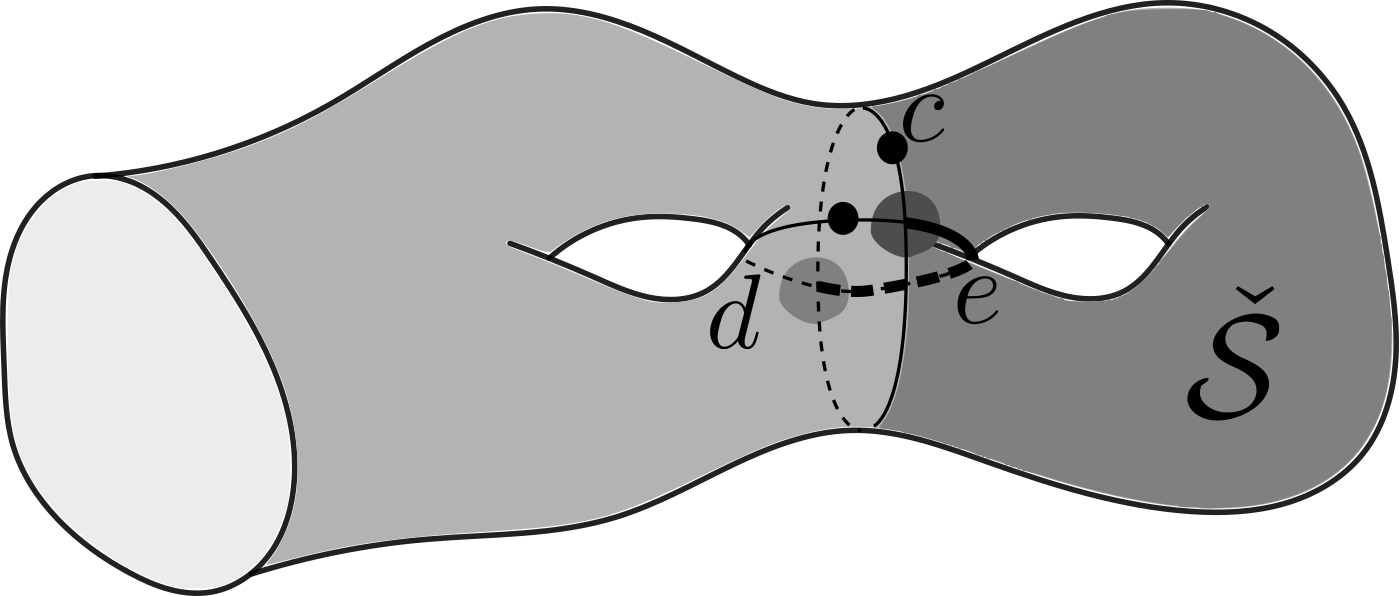
\includegraphics[scale=1]{figures/examplefive.pdf}
 \caption{}
\label{fig:examplefive}
\end{figure}

If we consider more than 2 points, the examples become more and more complicated, and proving the theorem with this geometric
approach seems rather difficult.